%% LyX 2.3.4.2 created this file.  For more info, see http://www.lyx.org/.
%% Do not edit unless you really know what you are doing.
\documentclass[english,dvipsnames,aspectratio=169]{beamer}
\usepackage{mathptmx}
\usepackage{eulervm}
\usepackage[T1]{fontenc}
\usepackage[latin9]{inputenc}
\usepackage{babel}
\usepackage{amstext}
\usepackage{amssymb}
\usepackage{graphicx}
\usepackage{ifthen}
\usepackage{xcolor}
\usepackage{xspace}
\usepackage{tikz}
\usetikzlibrary{tikzmark}
\usetikzlibrary{calc}
\usepackage{pgfplots}
%\pgfplotsset{compat=1.17}
\usepackage{booktabs}
\usepackage{xpatch}

\xpatchcmd{\itemize}
  {\def\makelabel}
  {\ifnum\@itemdepth=1\relax
     \setlength\itemsep{2ex}% separation for first level
   \else
     \ifnum\@itemdepth=2\relax
       \setlength\itemsep{1ex}% separation for second level
     \else
       \ifnum\@itemdepth=3\relax
         \setlength\itemsep{0.5ex}% separation for third level
   \fi\fi\fi\def\makelabel
  }
 {}
 {}

\ifx\hypersetup\undefined
  \AtBeginDocument{%
    \hypersetup{unicode=true,pdfusetitle,
 bookmarks=true,bookmarksnumbered=false,bookmarksopen=false,
 breaklinks=false,pdfborder={0 0 0},pdfborderstyle={},backref=false,colorlinks=true,
 allcolors=NYUPurple,urlcolor=LightPurple}
  }
\else
  \hypersetup{unicode=true,pdfusetitle,
 bookmarks=true,bookmarksnumbered=false,bookmarksopen=false,
 breaklinks=false,pdfborder={0 0 0},pdfborderstyle={},backref=false,colorlinks=true,
 allcolors=NYUPurple,urlcolor=LightPurple}
\fi

\makeatletter

%%%%%%%%%%%%%%%%%%%%%%%%%%%%%% LyX specific LaTeX commands.
%% Because html converters don't know tabularnewline
\providecommand{\tabularnewline}{\\}

%%%%%%%%%%%%%%%%%%%%%%%%%%%%%% Textclass specific LaTeX commands.
% this default might be overridden by plain title style
\newcommand\makebeamertitle{\frame{\maketitle}}%
% (ERT) argument for the TOC
\AtBeginDocument{%
  \let\origtableofcontents=\tableofcontents
  \def\tableofcontents{\@ifnextchar[{\origtableofcontents}{\gobbletableofcontents}}
  \def\gobbletableofcontents#1{\origtableofcontents}
}

%%%%%%%%%%%%%%%%%%%%%%%%%%%%%% User specified LaTeX commands.
\usetheme{CambridgeUS} 
\beamertemplatenavigationsymbolsempty


% Set Color ==============================
\definecolor{NYUPurple}{RGB}{87,6,140}
\definecolor{LightPurple}{RGB}{165,11,255}


\setbeamercolor{title}{fg=NYUPurple}
\setbeamercolor{frametitle}{fg=NYUPurple}

\setbeamercolor{background canvas}{fg=NYUPurple, bg=white}
\setbeamercolor{background}{fg=black, bg=NYUPurple}

\setbeamercolor{palette primary}{fg=black, bg=gray!30!white}
\setbeamercolor{palette secondary}{fg=black, bg=gray!20!white}
\setbeamercolor{palette tertiary}{fg=gray!20!white, bg=NYUPurple}

\setbeamertemplate{headline}{}
\setbeamerfont{itemize/enumerate body}{}
\setbeamerfont{itemize/enumerate subbody}{size=\normalsize}

\setbeamercolor{parttitle}{fg=NYUPurple}
\setbeamercolor{sectiontitle}{fg=NYUPurple}
\setbeamercolor{sectionname}{fg=NYUPurple}
\setbeamercolor{section page}{fg=NYUPurple}
%\setbeamercolor{description item}{fg=NYUPurple}
%\setbeamercolor{block title}{fg=NYUPurple}

\setbeamertemplate{blocks}[rounded][shadow=false]
\setbeamercolor{block body}{bg=normal text.bg!90!NYUPurple}
\setbeamercolor{block title}{bg=NYUPurple!30, fg=NYUPurple}



\AtBeginSection[]{
  \begin{frame}
  \vfill
  \centering
\setbeamercolor{section title}{fg=NYUPurple}
 \begin{beamercolorbox}[sep=8pt,center,shadow=true,rounded=true]{title}
    \usebeamerfont{title}\usebeamercolor[fg]{title}\insertsectionhead\par%
  \end{beamercolorbox}
  \vfill
  \end{frame}
}

\makeatother

\setlength{\parskip}{\medskipamount} 

\input ../macros

\begin{document}
\input ../rosenberg-macros

\title[CS-GA 2565]{Course Overview}
\author{Mengye Ren}
\date{September 5, 2023}
\institute{NYU}

\makebeamertitle
\mode<article>{Just in article version}

\begin{frame}{Contents}
\tableofcontents{}
\end{frame}

\section{Logistics}
\begin{frame}{Course Staff}
\begin{itemize}
\item Instructor:
    \begin{itemize}
        \item Mengye Ren
    \end{itemize}

\item Graders:
    \begin{itemize}
        \item Shreya Agarwal
        \item Jash Rathod
    \end{itemize}
\end{itemize}
\end{frame}

\begin{frame}{Logistics}
\begin{itemize}
\item Class webpage: \url{https://nyu-cs2565.github.io/2023-fall} 
\begin{itemize}
    \item Course materials (lecture slides, homeworks) will be made available on the website
\end{itemize}
\item Announcements via Brightspace
\item Discussion / questions on CampusWire\\
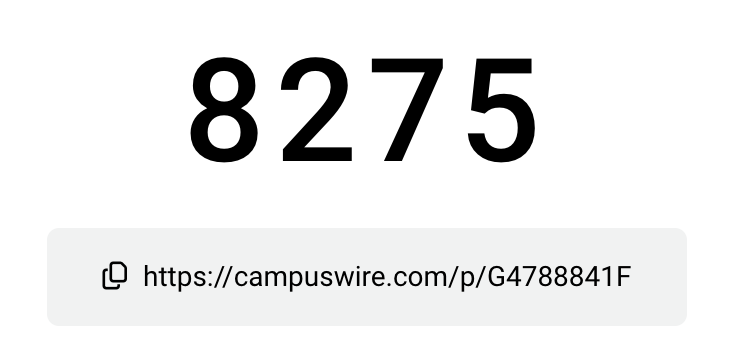
\includegraphics[width=0.4\textwidth,trim={0 5cm 0 0},clip]{figures/campuswire.png}
% \url{https://campuswire.com/p/G74AFD6C8}
% \item Sign up to Gradescope to submit homework assignments (entry code \textbf{DJZ86D})
\end{itemize}
\begin{itemize}
\item Office Hour: Tuesday 1:00-2:00 pm, Room 508, 60 Fifth Ave.
\end{itemize}
\end{frame}

\begin{frame}{Assessment}
\begin{itemize}
\item 4 assignments ($40\%$)
% \begin{itemize}
\item Midterm Exam ($30\%$)
\item Final Project ($30\%$)
\item Extra credits ($2\%$) answer other students' questions in a substantial and helpful way on Campuswire
\end{itemize}
\end{frame}
%
\begin{frame}{Homework}
\begin{itemize}
    \item Submit through Gradescope as a \textbf{PDF document}
    \item Late policy: You have 4 late days in total which can be used throughout the semester without penalty (see more details on website).

\item You can discuss with other students on the homework assignments, but:
\begin{itemize}
\item Write up the solutions and code on your own;
\item And list the names of the students you discussed each problem with.
\end{itemize}
\item If your solution or code is substantially similar to other students then it will be treated as plagiarism.

\end{itemize}
\end{frame}

\begin{frame}{Final Project}
\end{frame}


\begin{frame}{Prerequisites}
\begin{itemize}
\item Multivariate Calculus: partial derivatives/gradient.
\item Linear Algebra: vector/matrix manipulations, properties.
\item Probability Theory: common distributions; Bayes Rule.
\item Statistics: expectation, variance, covariance, median; maximum likelihood.
\item Programming: Python, numpy
\end{itemize}
\end{frame}


\section{Course Overview and Goals}
\begin{frame}{Syllabus (Tentative)}

12 weeks of instruction + 1 week midterm exam + 1 week project presentation
\begin{itemize}

\item 2 weeks: introduction to \textbf{machine learning}, \textbf{optimization}

\item 2 weeks: \textbf{Linear }methods for binary classification
and regression (also\textbf{ kernel methods)}

\item 2 weeks: \textbf{Probabilistic models}, \textbf{Bayesian}
methods

\item 1 week: \textbf{Multiclass} classification and introduction to \textbf{structured
prediction}

\item 3 weeks: \textbf{Nonlinear} methods (\textbf{trees}, \textbf{ensemble}
methods, and \textbf{neural networks})

\item 1 week: \textbf{Unsupervised} learning: \textbf{clustering} and \textbf{latent variable} models

\item 1 week: \textbf{Reinforcement} learning

\item More detailed schedule on the course website (still subject to change)
\end{itemize}
\end{frame}

\begin{frame}{The high level goals of the class}
\begin{itemize}
\item Our focus will be on the fundamental building blocks of machine learning
\item Prepare the fundamental toolkit -- fancy new methods are often combination of the techniques
\item Understand what kind of problems can ML help solve
\item Despite the large number of methods, understand the pros \& cons of each method, understand the motivation why we choose one method over the other
\item Apply ML in practical problems
\end{itemize}
\end{frame}

\begin{frame}{The level of the class}
\begin{itemize}
\item We will learn how to implement each ML algorithm \textbf{from scratch} using numpy alone, without any ML libraries.
\item Once we have implemented an algorithm from scratch once, we will use the sklearn version.
\end{itemize}
\end{frame}
\end{document}
